\section{Design Definition}
\label{sec:definition}

\begin{figure}[H]
\centering
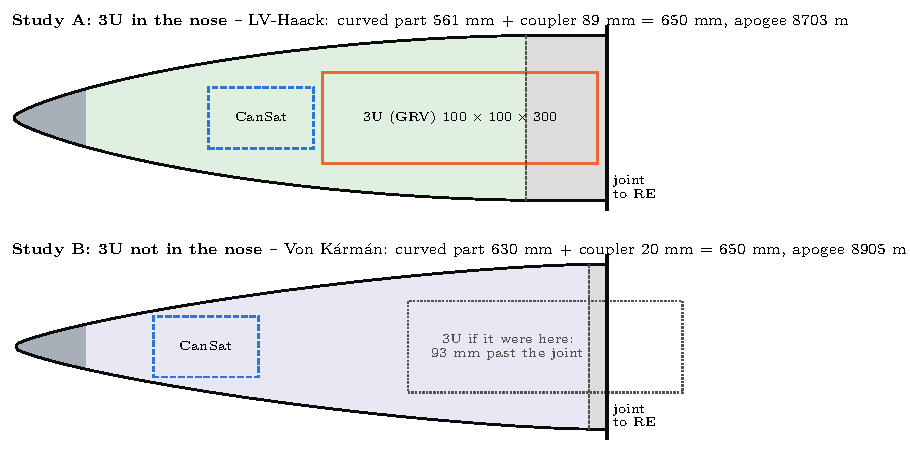
\includegraphics[width=\textwidth]{fig_tl_designs}
\caption{The two designs to scale (mm). Grey: tip and coupler cylinder; thick line: joint
to the RE bay; orange: 3U; blue dashed: CanSat; grey dotted (B): where the 3U would sit if it were in
the nose.}
\label{fig:designs}
\end{figure}

\begin{table}[H]
\centering
\caption{The two nose cones. Positions from the physical tip.}
\label{tab:final}
\small
\begin{tabular}{@{}>{\raggedright\arraybackslash}p{3.3cm}>{\raggedright\arraybackslash}p{6.0cm}>{\raggedright\arraybackslash}p{6.0cm}@{}}
\toprule
 & \textbf{A: 3U in the nose} & \textbf{B: 3U not in the nose} \\
\midrule
Profile & LV-Haack, Haack series $C = \tfrac13$ & Von K\'arm\'an, Haack series $C = 0$ \\
\multicolumn{3}{@{}l}{\quad Haack series: $y = \dfrac{R}{\sqrt\pi}\sqrt{\theta-\tfrac12\sin 2\theta + C\sin^3\theta}$,
$\theta=\arccos\!\left(1-\dfrac{2x}{L}\right)$, $x$ from the apex, $R = \SI{90}{mm}$} \\[4pt]
Curved length $L$ (to the theoretical apex) & \TLInLVHL{} ($L/D = \TLInLVHLD$); \TLInLVHPHYS{} physical & \TLOutVKL{} ($L/D = \TLOutVKLD$); \TLOutVKPHYS{} physical \\
Coupler cylinder & \TLInLVHC, full diameter, tangent & \TLOutVKC, full diameter, tangent \\
Total length & \SI{650}{mm} (\TLInLVHTOTPHYS{} physical) & \SI{650}{mm} (\TLOutVKTOTPHYS{} physical) \\
3U & front face at \TLInLVHXGRV; \TLInLVHLIN{} in the curved part, \TLInLVHINC{} in the cylinder & elsewhere in the vehicle \\
CanSat (needs \SI{115}{mm}) & \TLInLVHCAN{} of length with $r \geq \SI{39.2}{mm}$ ahead of the 3U & \TLOutVKCAN{} of length with $r \geq \SI{39.2}{mm}$ \\
Nose CP (Barrowman) & \TLInLVHXCP{} from the tip & \TLOutVKXCP{} from the tip \\
Apogee (model) & \TLInLVHAPO{} (\TLInLVHD); $M_{\max} = \TLInLVHMMAX$ & \TLOutVKAPO{} (\TLOutVKD); $M_{\max} = \TLOutVKMMAX$ \\
Static margin change & \TLInLVHDSM{} cal vs.\ the LVS nose & \TLOutVKDSM{} cal (nose only; without the 3U shift) \\
Both & \multicolumn{2}{p{12.2cm}}{\raggedright Tip: sphere $r_n = \SI{4.5}{mm}$. Diameter \SI{180}{mm}.} \\
Geometry files & {\footnotesize\TLInLVHFILE} & {\footnotesize\TLOutVKFILE} \\
\bottomrule
\end{tabular}
\end{table}

\subsection{CAD for the Fluent runs}

The six design points of Table~\ref{tab:designs} (three profiles, two studies) are exported as
solids of revolution in mm, $x$ from the physical tip, made of the blunted profile, the coupler
cylinder and a flat base at the joint: STEP (OpenCASCADE B-spline through 200 points), watertight
STL and the profile CSV. The STEP and CSV files are in \texttt{CFD/geometry\_650/} of the repository
(STL in \texttt{output/weisshorn\_650/total\_length/cad/}); the STEP volumes agree with the STL
within 0.1\,\%. They replace the \SI{810}{mm} geometry in the Fluent workflow note of the
\texttt{CFD} folder; the set-up, Mach numbers and meshing are unchanged.
